\chapter{Two-stage elections with multipartisan primary selection}
\label{sec:20}

\abstract*{}

\abstract{}

In a \emph{social choice} context, where decision objectives would match different political parties, Pareto efficient choice recommendations represent in fact \emph{multipartisan} social choices that could judiciously deliver the primary selection in a two stage election system.

To compute such Pareto efficient social choices we need to, first, convert a given linear voting profile (with polls) into a corresponding performance tableau.
 
\section{Converting voting profiles into performance tableaux}
\label{sec:20.1}

We shall illustrate this point with a voting profile we discussed already in Chapter \ref{sec:x}.
\begin{lstlisting}[caption={Example of a 3 parties voting profile},label=list:20.1]
>>> from votingProfiles import RandomLinearVotingProfile
>>> lvp = RandomLinearVotingProfile(numberOfCandidates=15,
...                         numberOfVoters=1000,
...                         WithPolls=True,
...                         partyRepartition=0.5,
...                         other=0.1,
...                         seed=0.9189670954954139)
>>> lvp
  *------- VotingProfile instance description ------*
   Instance class   : RandomLinearVotingProfile
   Instance name    : randLinearProfile
   Candidates       : 15
   Voters           : 1000
   Attributes       : ['name', 'seed', 'candidates',
             'voters', 'WithPolls', 'RandomWeights',
             'sumWeights', 'poll1', 'poll2',
             'other', partyRepartition,
             'linearBallot', 'ballot']
>>> lvp.showRandomPolls()
  Random repartition of voters
   Party_1 supporters : 460 (46.0%)
   Party_2 supporters : 436 (43.6%)
   Other voters       : 104 (10.4%)
  *---------------- random polls ----------------
   Party-1(46.0%) | Party-(43.6%)|  expected  
   ----------------------------------------------
    a06 : 19.91%  | a11 : 22.94%  | a06 : 15.00%
    a07 : 14.27%  | a08 : 15.65%  | a11 : 13.08%
    a03 : 10.02%  | a04 : 15.07%  | a08 : 09.01%
    a13 : 08.39%  | a06 : 13.40%  | a07 : 08.79%
    a15 : 08.39%  | a03 : 06.49%  | a03 : 07.44%
    a11 : 06.70%  | a09 : 05.63%  | a04 : 07.11%
    a01 : 06.17%  | a07 : 05.10%  | a01 : 05.06%
    a12 : 04.81%  | a01 : 05.09%  | a13 : 05.04%
    a08 : 04.75%  | a12 : 03.43%  | a15 : 04.23%
    a10 : 04.66%  | a13 : 02.71%  | a12 : 03.71%
    a14 : 04.42%  | a14 : 02.70%  | a14 : 03.21%
    a05 : 04.01%  | a15 : 00.86%  | a09 : 03.10%
    a09 : 01.40%  | a10 : 00.44%  | a10 : 02.34%
    a04 : 01.18%  | a05 : 00.29%  | a05 : 01.97%
    a02 : 00.90%  | a02 : 00.21%  | a02 : 00.51%
\end{lstlisting}
In this example (see Listing \ref{list:20.1} Lines 18-), we obtained 460 Party-1 supporters ($46\%$), 436 Party-2 supporters ($43.6\%$) and 104 other voters ($10.4\%$). Favorite candidates of Party-1 supporters, with more than $10\%$, appeared to be 'a06' ($19.91\%$), 'a07' ($14.27\%$) and 'a03' ($10.02\%$). Whereas for Party-2 supporters, favorite candidates appeared to be 'a11' ($22.94\%$), followed by 'a08' ($15.65\%$), 'a04' ($15.07\%$) and 'a06' ($13.4\%$).

We may convert this linear voting profile into a PerformanceTableau object where each political party matches to a decision objective.
\begin{lstlisting}[caption={Converting a voting profile into a performance tableau},label=list:20.2]
>>> lvp.save2PerfTab('votingPerfTab')
>>> from perfTabs import PerformanceTableau
>>> vpt = PerformanceTableau('votingPerfTab')
>>> vpt
  *------- PerformanceTableau instance description ---*
    Instance class   : PerformanceTableau
    Instance name    : votingPerfTab
    Actions          : 15
    Objectives       : 3
    Criteria         : 1000
    Attributes       : ['name', 'actions', 'objectives',
              'criteria', 'weightPreorder', 'evaluation']
>>> vpt.objectives
  OrderedDict([
    ('party0', {'name': 'other', 'weight': Decimal('104'),
     'criteria': ['v0003', 'v0008', 'v0011', ... ']}),
    ('party1', {'name': 'party 1', 'weight': Decimal('460'),
     'criteria': ['v0002', 'v0006', 'v0007', ...]}),
    ('party2', {'name': 'party 2', 'weight': Decimal('436'),
      'criteria': ['v0001', 'v0004', 'v0005', ... ]})
    ])
\end{lstlisting}
In Listing \ref{list:20.2} we first store the linear voting in a \texttt{PerformanceTableau} format (see Line 1). In Line 3, we reload this performance tableau data. The three parties of the linear voting profile represent three decision objectives and the 1000 voters are distributed as 10000 performance criteria according to the party they support.

\section{Multipartisan primary selection of eligible candidates}
\label{sec:20.2}

In order to operate now a \emph{primary multipartisan selection} of potential election winners, we compute the corresponding unopposed multiobjective outranking digraph (see Section \ref{sec:19.5}).
\begin{lstlisting}[caption={Computing unopposed multiobjective outranking situations},label=list:20.3]
>>> from outrankingDigraphs import \
...       UnOpposedBipolarOutrankingDigraph
>>> uog = UnOpposedBipolarOutrankingDigraph(vpt)
>>> uog
  *------- Object instance description ------*
    Instance class      : UnOpposedBipolarOutrankingDigraph
    Instance name       : unopposed_outrankings
    Actions             : 15
    Criteria            : 1000
    Size                : 34
    Oppositeness (%)    : 67.31
    Determinateness (%) : 57.61
    Valuation domain    : [-1.00;1.00]
    Attributes          : ['name', 'actions', 'valuationdomain',
                           'objectives', 'criteria', 'methodData',
                           'evaluation', 'order', 'runTimes',
                           'relation', 'marginalRelationsRelations',
                           'gamma', 'notGamma']
\end{lstlisting}
From the potential 105 pairwise outranking situations, we keep 34 positively validated outranking situations, leading to a degree of \emph{oppositeness} between political parties of $67.31\%$.

We may visualize the corresponding bipolar-valued relation table by orienting the list of candidates with the help of the initial and terminal prekernels.
\begin{lstlisting}[caption={Computing unopposed multiobjective outranking situations},label=list:20.4]
>>> uog.showPreKernels()
  *--- Computing preKernels ---*
   Dominant preKernels :
    ['a11', 'a06', 'a13', 'a15']
       independence :  0.0
       dominance    :  0.18
       absorbency   :  -0.66
       covering     :  0.43
   Absorbent preKernels :
    ['a02', 'a04', 'a14', 'a03']
       independence :  0.0
       dominance    :  0.0
       absorbency   :  0.37
       covered      :  0.46
>>> orientedCandidatesList = ['a06','a11','a13','a15',\
...         'a01','a05','a07','a08','a09','a10','a12',\
...         'a02','a03','a04','a14']
>>> uog.showHTMLRelationTable(\
...    actionsList=orientedCandidatesList,\
...    tableTitle='Unopposed three-partisan outrankings')
\end{lstlisting}
\begin{figure}[h]
%\sidecaption
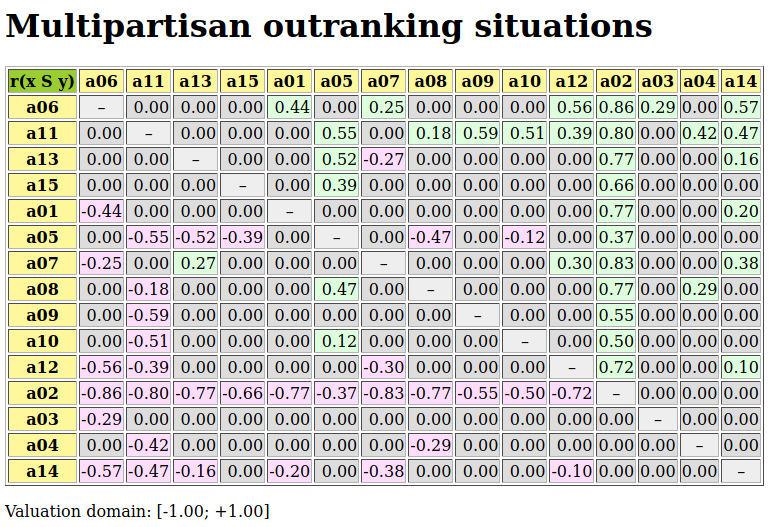
\includegraphics[width=12cm]{Figures/unOpposedOutrankings.png}
\caption{Relation table of multipartisan outranking digraph} 
\label{fig:20.1}       % Give a unique label
\end{figure}

In Fig. \ref{fig:20.1}, we may notice that the dominating outranking prekernel ['a06', 'a11', 'a13', 'a15'] gathers in fact a multipartisan selection of potential election winners. It is worthwhile noticing that in the majority margins obtained from a linear voting profile do verify the zero-sum rule: $\big(\,r(x \succsim y) \,+\, r(y \succsim x) \;=\; 0.0\,\big)$. To each positive outranking situation corresponds indeed an equivalent negative converse situation and the resulting outranking and strict outranking digraphs are the same.

\section{Secondary election winner determination}
\label{sec:20.3}

When restricting now, in a secondary election stage, the set of eligible candidates to this dominating prekernel, we may compute the actual best social choice.
\begin{lstlisting}[caption={Recommending the secondary election winner},label=list:20.5]
>>> from outrankingDigraphs import BipolarOutrankingDigraph
>>> g2 = BipolarOutrankingDigraph(vpt,\
..          actionsSubset=['a06','a11','a13','a15'])
>>> g2.showRelationTable(ReflexiveTerms=False)
  * ---- Relation Table -----
     r    | 'a06'  'a11'  'a13'  'a15'   
    ------|----------------------------
    'a06' |   -    +0.10  +0.48  +0.52  
    'a11' | -0.10    -    +0.27  +0.29  
    'a13' | -0.48  -0.27    -    +0.19  
    'a15' | -0.52  -0.29  -0.19    -   
    Valuation domain: [-1.0; 1.0]
>>> g2.computeCondorcetWinners()
  ['a06']
>>> g2.computeCopelandRanking()
  ['a06', 'a11', 'a13', 'a15']
\end{lstlisting}
Candidate 'a06' appears clearly to be the winner of this election. Notice by the way that the restricted pairwise outranking relation shown in Listing \ref{list:20.5} represents a linear ordering of the preselected candidates.

We may eventually check the quality of this best choice by noticing that candidate 'a06' represents indeed the \emph{simple majority}, the \emph{instant-run-off}, the \Borda, as well as the \Condorcet winner of the initially given linear voting profile $lvp$.
\begin{lstlisting}
>>> lvp.computeSimpleMajorityWinner()
  ['a06']
>>> lvp.computeInstantRunoffWinner()
  ['a06']
>>> lvp.computeBordaWinners()
  ['a06']
>>> from votingProfiles import MajorityMarginsDigraph
>>> cd = MajorityMarginsDigraph(lvp)
>>> cd.computeCondorcetWinners()
  ['a06']
\end{lstlisting}

In our example voting profile here, the multipartisan primary selection stage appears quite effective in reducing the number of eligible candidates to four out of a set of 15 candidates without btw rejecting the actual winning candidate.

\section{Multipartisan preferences in divisive politics}
\label{sec:20.4}

However, in a very \emph{divisive} two major parties system, like in the US, where preferences of the supporters of one major party appear to be very opposite to the preferences of the supporters of the other major party, the multipartisan outranking digraph will become nearly indeterminate.

In Listing \ref{list:20.6} below we generate such a divisive kind of linear voting profile with the help of the \texttt{DivisivePolitics} flag \footnote{The \texttt{RandomLinearVotingProfile} constructor provides a \texttt{DivisivePolitics} flag (\emph{False} by default) for generating random linear voting profiles based on a divisive polls strucure.} (see Lines 4 and 13-19). When now converting the voting profile into a performance tableau (Lines 20-21), we may compute the corresponding unopposed outranking digraph.
\begin{lstlisting}[caption={A divisive two-party example of a random linear voting profile},label=list:20.6]
>>> from votingProfiles import RandomLinearVotingProfile		     
>>> lvp = RandomLinearVotingProfile(\
...      numberOfCandidates=7,numberOfVoters=500,\
...      WithPolls=True, partyRepartition=0.4,other=0.2,\
...      DivisivePolitics=True, seed=1)
>>> lvp.showRandomPolls()
  Random repartition of voters
   Party-1 supporters : 240 (48.00%)
   Party-2 supporters : 160 (32.00%)
   Other voters       : 100 (20.00%)
  *---------------- random polls -------------
   Party_1(48.0%) | Party_2(32.0%) | expected  
   -------------------------------------------
   a2 : 30.84%    |  a1 : 30.84%   | a2 : 15.56%
   a3 : 23.67%    |  a4 : 23.67%   | a3 : 12.91%
   a7 : 17.29%    |  a6 : 17.29%   | a7 : 11.43%
   a5 : 11.22%    |  a5 : 11.22%   | a1 : 11.00%
   a6 : 09.79%    |  a7 : 09.79%   | a6 : 10.23%
   a4 : 04.83%    |  a3 : 04.83%   | a4 : 09.89%
   a1 : 02.37%    |  a2 : 02.37%   | a5 : 08.98%
>>> lvp.save2PerfTab('divisiveExample')
>>> dvp = PerformanceTableau('divisiveExample')
>>> from outrankingDigraphs import \
...        UnOpposedBipolarOutrankingDigraph
>>> uodg = UnOpposedBipolarOutrankingDigraph(dvp)
>>> uodg
  *------- Object instance description ------*
   Instance class : UnOpposedBipolarOutrankingDigraph
   Instance name  : unopposed_outrankings
   Actions        : 7
   Criteria       : 500
   Size           : 0
   Oppositeness (%)    : 100.00
   Determinateness (%) : 50.00
   Valuation domain    : [-1.00;1.00]
\end{lstlisting}
With an oppositeness degree of $100.0\%$ (see Listing \ref{list:20.6} Lines 31-32), the preferential disagreement between the political parties is complete, and the unopposed outranking digraph $uodg$ becomes completely indeterminate as shown in the relation table below.
\begin{lstlisting}
>>> uodg.showRelationTable(ReflexiveTerms=False)
  * ---- Relation Table -----
   r   | 'a1'   'a2'  'a3'  'a4'  'a5'  'a6'  'a7'   
  -----|------------------------------------------
  'a1' |   -   +0.00 +0.00 +0.00 +0.00 +0.00 +0.00  
  'a2' | +0.00   -   +0.00 +0.00 +0.00 +0.00 +0.00  
  'a3' | +0.00 +0.00   -   +0.00 +0.00 +0.00 +0.00  
  'a4' | +0.00 +0.00 +0.00   -   +0.00 +0.00 +0.00  
  'a5' | +0.00 +0.00 +0.00 +0.00   -   +0.00 +0.00  
  'a6' | +0.00 +0.00 +0.00 +0.00 +0.00   -   +0.00  
  'a7' | +0.00 +0.00 +0.00 +0.00 +0.00 +0.00   -   
  Valuation domain: [-1.0; 1.0]
\end{lstlisting}      

As a consequence, a multipartisan primary selection, computed with a \texttt{showBestChoiceRecommendation()} method,  will keep the complete initial set of eligible candidates and, hence, becomes \emph{ineffective} (see Listing \ref{list:20.7} Line 6).
\begin{lstlisting}[caption={Example of ineffective primary multipartisan selection},label=list:20.7]
>>> uodg.showBestChoiceRecommendation()
  Rubis best choice recommendation(s) (BCR)
   (in decreasing order of determinateness)   
   Credibility domain: [-1.00,1.00]
   === >> ambiguous choice(s)
    choice              : ['a1','a2','a3','a4','a5','a6','a7']
    independence        : 0.00
    dominance           : 1.00
    absorbency          : 1.00
    covered (%)         : 100.00
    determinateness (%) : 50.00
     - most credible action(s) = { }
\end{lstlisting}

With such kind of divisive voting profile, there may indeed not always exist an obvious winner. In Listing \ref{list:20.8} below, we see, for instance, that the simple majority winnner is 'a2' (Line 2), whereas the instant-run-off winner is 'a6' (Line 4).
\begin{lstlisting}[caption={Example of non obvious secondary selection},label=list:20.8]
>>> lvp.computeSimpleMajorityWinner()
  ['a2']
>>> lvp.computeInstantRunoffWinner()
  ['a6']
>>> from votingProfiles import MajorityMarginsDigraph
>>> cg = MajorityMarginsDigraph(lvp)
>>> cg.showRelationTable(ReflexiveTerms=False)
  * ---- Relation Table -----
    r()  |  'a1' 'a2' 'a3' 'a4' 'a5' 'a6' 'a7'	  
   ------|------------------------------------
    'a1' |   -   -68  -90  -46  -68  -88  -84	 
    'a2' |  +68   -   -32  +80  +46   -6  -24	 
    'a3' |  +90  +32   -   +58  +46   +4   +8	 
    'a4' |   +4  -80  -58   -   -16  -68  -72	 
    'a5' |  +68  -46  -46  +16	 -   -26  -64	 
    'a6' |  +88   +6   -4  +68	+26   -    -2	 
    'a7' |  +84  +24   -8  +72	+64   +2   - 	 
Valuation domain: [-500;+500]
>>> cg.computeCondorcetWinners()
  ['a3']
>>> lvp.computeBordaWinners()
  ['a3','a7']
>>> cg.computeCopelandRanking()
  ['a3', 'a7', 'a6', 'a2', 'a5', 'a4', 'a1']
\end{lstlisting}
But in our example here, we are lucky. When constructing with the pairwise majority margins digraph (Line 6), a \Condorcet winner, namely 'a3' becomes apparent (Lines 13,20), which is also one of the two \Borda winners (Line 22). More interesting even is to notice that the apparent majority margins digraph models in fact a linear ranking ['a3','a7','a6','a2','a5','a4','a1'] of all the eligible candidates, as shown with a \Copeland ranking rule (Line 24).

We may eventually visualize in Fig. \ref{fig:20.2} this linear ranking with a graphviz drawing where we drop all transitive arcs (Line 1) and orient the drawing with \Condorcet winner 'a3' and loser 'a1' (Line 2 below).
\begin{lstlisting}
>>> cg.closeTransitive(Reverse=True)
>>> cg.exportGraphViz('divGraph',\
...            bestChoice=['a3'],worstChoice=['a1'])
  *---- exporting a dot file for GraphViz tools ---------*
   Exporting to divGraph.dot
   dot -Grankdir=BT -Tpng divGraph.dot -o divGraph.png
\end{lstlisting}
\begin{figure}[h]
\sidecaption
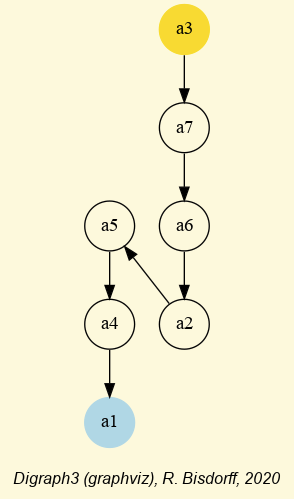
\includegraphics[width=5cm]{Figures/divGraph.png}
\caption{The linear ranking moddelled by the majority margins digraph.} 
\label{fig:20.2}       % Give a unique label
\end{figure}

The last Chapter \ref{sec:21} propose eventually a biploar approval voting system which could help healing a society who is facing important social choices in an excessive divisive political system.